% Copyright © 2015 Martin Ueding <dev@martin-ueding.de>

\documentclass[11pt, english, fleqn, DIV=15, headinclude, BCOR=1cm]{scrartcl}

\usepackage[bibatend, color]{../header}

\usepackage{tikz}

\usepackage[tikz]{mdframed}
\newmdtheoremenv[%
    backgroundcolor=black!5,
    innertopmargin=\topskip,
    splittopskip=\topskip,
]{theorem}{Theorem}[section]

\hypersetup{
    pdftitle=
}

\newcounter{totalpoints}
\newcommand\punkte[1]{#1\addtocounter{totalpoints}{#1}}

\newcounter{problemset}
\setcounter{problemset}{4}
\date{2015-04-29}

\subject{Geometry in Physics}
\ihead{Geometry in Physics -- Problem Set \arabic{problemset}}

\title{Problem Set \arabic{problemset}}

\publishers{Group 1 -- Jens Boos}
\ofoot{Group 1 -- Jens Boos}

\author{
    Martin Ueding \\ \small{\href{mailto:mu@martin-ueding.de}{mu@martin-ueding.de}}
    \and
    Paul Manz \\ \small{\href{mailto:paul.manz@dreiacht.de}{paul.manz@dreiacht.de}}
}
\ifoot{Martin Ueding, Paul Manz}

\ohead{\rightmark}

\usepackage{multicol}

\renewcommand\thesubsection{\thesection.\alph{subsection}}

\begin{document}

\maketitle

\vspace{3ex}

\begin{center}
    \begin{tabular}{rrr}
        problem & achieved points & possible points \\
        \midrule
        \nameref{homework:1} & & \punkte{10} \\
        \nameref{homework:2} & & \punkte{10} \\
        \nameref{homework:3} & & \punkte{10} \\
        \nameref{homework:4} & & \punkte{20} \\
        \midrule
        Total & & \arabic{totalpoints}
    \end{tabular}
\end{center}

\section{Visualization of differential forms}
\label{homework:1}

\subsection{Visualization}

The forms can be visualized in the dual space. In the dual space, there should
not be a problem by visualizing them with vectors. Vectors are translationally
invariant, so we can draw them anywhere, just like it is done on the problem
set. All four forms are shown in Figure~\ref{fig:forms-dual}.

\begin{figure}[htbp]
    \centering
    \begin{tikzpicture}[scale=2]
        \draw[->] (-.3, 0) -- (2, 0) node[right] {$\dif x^1$};
        \draw[->] (0, -.3) -- (0, 2) node[above] {$\dif x^1$};
        %
        \draw (1, .1) -- (1, -.1) node[below] {$1$};
        \draw (.1, 1) -- (-.1, 1) node[left] {$1$};
        %
        \draw[very thick, ->] (2.2, .4) -- ++(1, 0) node[midway, sloped, above] {$\dif x^1$};
        \draw[very thick, ->] (3, 1) -- ++(0, 1) node[midway, sloped, above] {$\dif x^2$};
        %
        \draw[very thick, ->] (0, 0) -- ++(30:2) node[midway, sloped, above] {$\dif r$};
        \draw[very thick, ->] (30:2) -- ++(120:.5) node[midway, sloped, above] {$\dif \phi$};
    \end{tikzpicture}
    \caption{%
        Visualization of $\dif x^1$, $\dif x^2$, $\dif r$ and $\dif \phi$ in
        the dual space.
    }
    \label{fig:forms-dual}
\end{figure}

Using the metric, which we probably have in standard $\R^2$, the arrows in
Figure~\ref{fig:forms-dual} could also be interpreted as the vectors $[\dif
x^1]^\sharp$. The Hodge dual is another way to visualize these. In components,
this is defined as
\[
    [\hodge \omega]^{i\ldots k} := \epsilon^{i\ldots kl\ldots n} \omega_{l
    \ldots n}.
\]
In the case of two dimensions this is just
\[
    [\hodge \omega]^i = \epsilon^{ij} \omega_j.
\]
Since $\epsilon^{12} = 1$ and $\epsilon^{21} = -1$, this is means that
\[
    [\hodge \omega]^1 = \omega_2
    \eqnsep
    [\hodge \omega]^2 = - \omega_1
\]
which corresponds to a rotation by $-\piup/2$. That is shown in
Figure~\ref{fig:forms}.

\begin{figure}[htbp]
    \centering
    \begin{tikzpicture}[scale=2]
        \draw[->] (-.3, 0) -- (2, 0) node[right] {$x^1$};
        \draw[->] (0, -2) -- (0, .3) node[above] {$x^1$};
        %
        \draw (1, .1) -- (1, -.1) node[below] {$1$};
        \draw (.1, -1) -- (-.1, -1) node[left] {$-1$};
        %
        \draw[very thick, ->] (2.2, -.4) -- ++(0, -1) node[midway, sloped, above]
        {$\hodge \dif x^1$};
        \draw[very thick, ->] (3, -1) -- ++(1, 0) node[midway, sloped, above]
        {$\hodge \dif x^2$};
        %
        \draw[very thick, ->] (0, 0) -- ++(-60:2) node[midway, sloped, above]
        {$\hodge \dif r$};
        \draw[very thick, ->] (-60:2) -- ++(30:.5) node[midway, sloped, above]
        {$\hodge \dif \phi$};
    \end{tikzpicture}
    \caption{%
        Visualization of $\hodge \dif x^1$, $\hodge \dif x^2$, $\hodge \dif r$
        and $\hodge \dif \phi$ in the regular space.
    }
    \label{fig:forms}
\end{figure}

\paragraph{Transformation of $\dif r$ into Cartesian coordinates}

The forms given in polar coordinates have to be transformed into Cartesian
coordinates to draw them into the Cartesian plot. Although the representation
of $\dif r$ in Cartesian coordinates seems “obvious”, we would like to engage
the full machinery of pullbacks and pushforwards in order to see whether we
understood the concepts correctly.

The transformation which brings us from Cartesian to polar coordinates is given
by
\begin{align*}
    \varphi \colon &\R^2_\text{Cartesian} \to \R^2_\text{polar} \\
                &x \ev_x + y \ev_y \mapsto \sqrt{x^2 + y^2} \, \ev_r + \arccos\del{\frac xr}
    \ev_\phi,
\end{align*}
although it is not well defined for all angles $\phi$. As long as we restrict
this to the first quadrant, everything is fine. Let us restrict this to the
open set $(0, \infty) \times (0, \infty)$ to make it easier. Then $\varphi$ is
a diffeomorphism.

Now we use a pullback which will let us bring tensors the other way around.
This is best expressed more formally:
\[
    \varphi^* \colon T_{\varphi(\xi)}\R^2_\text{polar} \to
    T_{\xi}\R^2_\text{Cartesian}
\]
$\xi$ is a point given in Cartesian coordinates. The components of a tensor
$\tens\omega$ then transform like the following: \parencite[(A.1.16)]{Metsch/physics754}
\[
    [\varphi^* \omega]^{\nu_1 \ldots}{}_{\mu_1\ldots}(\xi) =
    \omega^{\alpha_1 \ldots}{}_{\beta_1\ldots} (\varphi(\xi))
    \pd{y^{\beta_1}}{x^{\mu_1}} \cdots
    \pd{x^{\nu_1}}{y^{\alpha_1}} \cdots
    \eqnsep
    \vec y := \vec\varphi(\xi).
\]

With our given 1-form, this collapses to a single lower index:
\begin{align*}
    [\varphi^* \omega]_i(\xi)
    &= \omega_j(\varphi(\xi)) \pd{\varphi^j}{x^i}(\xi).
    \intertext{%
        $\omega$ is just $\dif r$, so we have the components $\omega_r = 1$ and
        $\omega_\phi = 0$. $r$ is not an index which takes on numbers, but we
        rather want it to be interpreted that $j \in \{r, \phi\}$. This is a
        bad overloading of symbols, but we hope that it is somewhat
        decipherable. Since there is only one component in $\omega$ the
        equation simplifies to
    }
    &= 1 \cdot \pd{\varphi^r}{x^i}(\xi).
    \intertext{%
        Using the explicit form of the map $\vec \varphi$, the partial
        derivatives are
    }
    &= \sbr{\frac{x_i}{\sqrt{x^2 + y^2}}}_{\xi}.
\end{align*}
This is now expressed in terms of Cartesian coordinates. It simplifies
to use the polar coordinates to write this more compact. Then we have
\[
    [\varphi^* \dif r]_i \dif x^i
    = \dif r
    = \cos(\phi) \dif x + \sin(\phi) \dif y.
\]

\paragraph{Conversion of $\dif \phi$}

Using the same derivation we can derive an expression for $\dif \phi$:
\begin{align*}
    [\varphi^* \dif \phi]_i(\xi)
    &= \dif \phi_j(\varphi(\xi)) \pd{\varphi^j}{x^i}(\xi) \\
    &= 1 \cdot \pd{\varphi^\phi}{x^i}(\xi)
\end{align*}
The derivatives are given by:
\[
    \pd{\varphi^\phi}{x} = - \frac{y}{r^2} = - \frac{\sin(\phi)}r
    \eqnsep
    \pd{\varphi^\phi}{y} = \frac{x}{r^2} = \frac{\cos(\phi)}r
\]
Therefore
\[
    \dif \phi = - \frac{\sin(\phi)}r \, \dif x + \frac{\cos(\phi)}r \, \dif y.
\]

\subsection{Values of 1-forms on vectors}

\paragraph{Values}

The vectors given in the image are:
\[
    \vec v_1 = \begin{pmatrix} 0 \\ 1 \end{pmatrix}
    \eqnsep
    \vec v_2 = \begin{pmatrix} -1 \\ -1 \end{pmatrix}
    \eqnsep
    \vec v_3 = \begin{pmatrix} 1 \\ -1 \end{pmatrix}
\]

The form $\omega_3$ needs a step of preparation.
\[
    \omega_3 = \dif r^2 = 2 r \dif r
\]

Then we can compute:
\begin{gather*}
    \omega_1(\vec v_1) = \dif x^1 (\partial_2) = 0 \\
    \omega_1(\vec v_2) = \dif x^1 (-\partial_1-\partial_2) = -1 \\
    \omega_1(\vec v_3) = \dif x^1 (\partial_1-\partial_2) = 1 \\
    \omega_2(\vec v_1) = x^1 \, \dif x^2 (\partial_2) = x^1 \\
    \omega_2(\vec v_2) = x^1 \, \dif x^2 (-\partial_1-\partial_2) = -x^1 \\
    \omega_2(\vec v_3) = x^1 \, \dif x^2 (\partial_1-\partial_2) = - x^1  \\
    \omega_3(\vec v_1) = 2 r \dif r (-\partial_1-\partial_2) = 2 r \sin(\phi) \\
    \omega_3(\vec v_2) = 2 r \dif r (\partial_1-\partial_2) = - 2 r
    \sbr{\cos(\phi) + \sin(\phi)} \\
    \omega_3(\vec v_3) = 2 r \dif r (\partial_1-\partial_2) = 2 r
    \sbr{\cos(\phi) - \sin(\phi)}
\end{gather*}

Everything is summarized in Table~\ref{tab:values}.

\begin{table}[htbp]
    \centering
    \begin{tabular}{c|ccc}
        & $\vec v_1$ & $\vec v_2$ & $\vec v_3$ \\
        \midrule
        $\omega_1$ & $0$ & $-1$ & $1$ \\
        $\omega_2$ & $x^1$ & $- x^1$ & $- x^1$ \\
        $\omega_3$ & $2 r \sin(\phi)$ & $- 2 r
        \sbr{\cos(\phi) + \sin(\phi)}$ & $2 r
        \sbr{\cos(\phi) - \sin(\phi)}$ \\
    \end{tabular}
    \caption{%
        Summary of value of the 1-forms on the vectors.
    }
    \label{tab:values}
\end{table}

\paragraph{Geometric interpretation}

1-forms are densities in one dimension. Examples are the force $\vec F$ or the
electric field $\vec E$. So the value $\omega(\vec v)$ then gives the amount of
“work” done along the tangential vector $\vec v$ against the “force” $\omega$.

If one uses the metric and computes the vector which are dual to the 1-forms,
this is a scalar product. But we think that this is exactly what is \emph{not}
wanted here.

\subsection{Values of 2-forms on parallelograms}

For your convenience, all the results are aggregated in
Table~\ref{tab:values2}. The derivations are following, of course.

\begin{table}[htbp]
    \centering
    \begin{tabular}{c|ccc}
        & $(\vec v_1, \vec w_1)$ & $(\vec v_2, \vec w_2)$ & $(\vec v_3, \vec w_3)$ \\
        \midrule
        $\eta_1$ & $1$ & $2$ & $-1$ \\
        $\eta_2$ & $x^1+x^2$ & $2\sbr{x^1+x^2}$ & $-\sbr{x^1+x^2}$ \\
        $\eta_3$ & $1$ & $2$ & $-1$
    \end{tabular}
    \caption{%
        Summary of value of the 2-forms on the vector pairs.
    }
    \label{tab:values2}
\end{table}

\paragraph{First form}

The first value is given by
\begin{align*}
    \eta_1(\vec v_1, \vec w_1)
    &= \sbr{\dif x^1 \wedge \dif x^2}(\vec v_1, \vec w_1) \\
    &= \sbr{\dif x^1 \wedge \dif x^2} \del{
        \begin{pmatrix}
            1 \\ 0
        \end{pmatrix},
        \begin{pmatrix}
            1 \\ 1
        \end{pmatrix}
    } \\
    &= \sbr{\dif x^1 \wedge \dif x^2} \del{\ev_1, \ev_1 + \ev_2} \\
    &= \sbr{\dif x^1 \wedge \dif x^2} \del{\ev_1, \ev_1}
    + \sbr{\dif x^1 \wedge \dif x^2} \del{\ev_1, \ev_2}. \\
    \intertext{%
        The first part is zero. The differential form must be antisymmetric in
        its arguments. The second summand is 1.
    }
    &= 1.
\end{align*}

The second one:
\begin{align*}
    \eta_1(\vec v_2, \vec w_2)
    &= \sbr{\dif x^1 \wedge \dif x^2} \del{\ev_1 - \ev_2, 2 \ev_2} \\
    &= 2 \sbr{\dif x^1 \wedge \dif x^2} \del{\ev_1, \ev_2}
    - 2 \sbr{\dif x^1 \wedge \dif x^2} \del{\ev_2, \ev_2}
    \intertext{%
        Here the first term is one, the second term is zero.
    }
    &= 2
\end{align*}

And the last one with $\eta_1$.
\begin{align*}
    \eta_1(\vec v_3, \vec w_3)
    &= \sbr{\dif x^1 \wedge \dif x^2} \del{- \ev_1, \ev_2} \\
    &= - \sbr{\dif x^1 \wedge \dif x^2} \del{\ev_1, \ev_2} \\
    &= - 1
\end{align*}

\paragraph{Second form}

For 2-forms, there is just one basis element, namely $\dif x^1 \wedge \dif
x^2$. So all 2-forms are just scalar densities and cannot depend on the
direction. 2-forms are also Hodge dual to scalars, which also do not depend on
the direction. Therefore, all those 2-forms are scalar multiples of each other.
This makes it really easy to compute the remaining values.

First we have to rewrite $\eta_2$ in terms of this \emph{one} basis value. We
think that this form of $\eta_2$ is just given this way to encourage people to
think before doing a lot of calculations. The wedge product is antisymmetric,
so this can be written more compact as
\[
    \eta_2
    = \sbr{x^1 \, \dif x^1 \wedge \dif x^2 - x^2 \, \dif x^2 \wedge \dif x^1}
    = \sbr{ x^1 + x^2} \sbr{\dif x^1 \wedge \dif x^2}
    = \sbr{ x^1 + x^2} \eta_1.
\]
Therefore, the values are all the same, just multiplied with that factor.

\paragraph{Third form}

The third form is a 2-form as well, so it must be a scalar multiple of $\dif
x^1 \wedge \dif x^2$.
\begin{align*}
    \eta_3
    &= r \, \dif r \wedge \dif \phi
    \intertext{%
        Now we use the expressions in the Cartesian dual basis that we have
        derived previously.
    }
    &= r \sbr{\cos(\phi) \dif x + \sin(\phi) \dif y} \wedge
    \sbr{-\frac{\sin(\theta)}r \dif x + \frac{\cos(\phi)}r \dif y}
    \intertext{%
        We would get four terms in the multiplication. There are only two
        nonzero ones since the wedge product is antisymmetric and the first and
        last terms would cancel then. We only keep the inner and outer terms.
    }
    &= \cos(\phi)^2 \dif x \wedge \dif y - \sin(\phi)^2 \dif y \wedge
    \dif x \\
    \intertext{%
        Here we use the antisymmetry of the wedge product.
    }
    &= \cos(\phi)^2 \dif x \wedge \dif y + \sin(\phi)^2 \dif x \wedge
    \dif y \\
    \intertext{%
        Now we can factor out the basis element of the 2-forms.
    }
    &= \sbr{\cos(\phi)^2 + \sin(\phi)^2} \dif x \wedge \dif y \\
    &= \dif x \wedge \dif y
\end{align*}
So this is exactly $\eta_1$ and since the 2-forms cannot depend on direction in
$\R^2$, the values when acting on the vector pairs are exactly the as for
$\eta_1$.

\section{Straight forward calculations}
\label{homework:2}

\subsection{Forms and inner derivative}

\paragraph{Exterior derivative}

The exterior derivative of $\theta$ can be computed using the graded Leibniz
rule.
\begin{align*}
    \dif \theta
    &= \dif \sbr{\exp(x^1 x^2) \dif x^1 - \dif x^2} \\
    \intertext{%
        We use the linearity of the exterior derivative.
    }
    &= \dif \, \big[\underbrace{\exp(x^1 x^2)}_\text{0-form} \underbrace{\dif
    x^1}_\text{1-form} \big] - \dif \sbr{\dif x^2} \\
    \intertext{%
        Now we can use the graded Leibniz rule.
    }
    &= \dif \exp(x^1 x^2) \wedge \dif x^1 + [-1]^0 \exp(x^1 x^2) \wedge \dif^2
    x^1
    \intertext{%
        The $[-1]^0$ comes from the graded Leibniz rule. The $\dif^2 x^1 = 0$,
        so we can drop the second summand. We now have to apply the chain rule
        for the exponential function.
    }
    &= \exp(x^1 x^2) \dif[x^1 x^2] \wedge \dif x^1
    \intertext{%
        The square bracket now contains a product of two 0-forms. We apply the
        graded Leibniz rule again.
    }
    &= \exp(x^1 x^2) \sbr{\dif x^1 \wedge x^2 + [-1]^0 x^1 \wedge \dif x^2}
    \wedge \dif x^1 \\
    &= \exp(x^1 x^2) \sbr{x^2 \dif x^1 + x^1 \dif x^2} \wedge \dif x^1 \\
    \intertext{%
        The only non-zero term is the product of $\dif x^2$ with $\dif x^1$. We
        are left with a single term.
    }
    &= \exp(x^1 x^2) x^1 \dif x^2 \wedge \dif x^1 \\
    \intertext{%
        As a last step we use the antisymmetry of the wedge product.
    }
    &= - \exp(x^1 x^2) x^1 \dif x^1 \wedge \dif x^2
\end{align*}

\paragraph{Wedge product}

\begin{align*}
    \omega \wedge \theta
    &= \sbr{2x^1 x^2 \dif x^1 + \sbr{[x^1]^2 + 3} \dif x^2} \wedge
    \sbr{\exp(x^1 x^2) \dif x^1 - \dif x^2}
    \intertext{%
        Again, there are only two interesting terms.
    }
    &= - 2x^1 x^2 \dif x^1 \wedge \dif x^2 + \sbr{[x^1]^2 + 3} \exp(x^1 x^2) \dif
    x^2 \wedge \dif x^1
    \intertext{%
        Using the antisymmetry, this can be written as a scalar multiple of the
        one basis element.
    }
    &= \sbr{- 2x^1 x^2 - \sbr{[x^1]^2 + 3} \exp(x^1 x^2)} \dif x^1 \wedge \dif x^2
\end{align*}

\paragraph{Inner derivative}

First we need to have the components of our 2-form $\dif \theta$:
\[
    [\dif \theta]_{12} = - [\dif \theta]_{21} =
    - \exp(x^1 x^2) x^1
    \eqnsep
    [\dif \theta]_{11} = [\dif \theta]_{22} = 0.
\]
Now we can apply the inner derivative:
\[
    [i_{\vec X}(\dif \theta)]_k = X^j [\dif \theta]_{jk}
\]
In order to get a 1-form out, we need to contract the components with the basis
elements of the dual space again.
\begin{align*}
    i_{\vec X}(\dif \theta)
    &= X^j [\dif \theta]_{jk} \dif x^k
    \intertext{%
        The only nonzero components are then:
    }
    &= X^1 [\dif \theta]_{12} \dif x^2 + X^2 [\dif \theta]_{21} \dif x^1
    \intertext{%
        We use the antisymmetry of the 2-form.
    }
    &= X^1 [\dif \theta]_{12} \dif x^2 - X^2 [\dif \theta]_{12} \dif x^1
    \intertext{%
        Now we can extract the components of the 2-form.
    }
    &= [\dif \theta]_{12} \sbr{X^1 \dif x^2 - X^2 \dif x^1}
    \intertext{%
        Now we insert the explicit form of the components.
    }
    &= - \exp(x^1 x^2) x^1 \sbr{\dif x^2 - [x^1]^2 x^2 \dif x^1}
\end{align*}

\subsection{Pullback}

We have a map which maps from polar coordinates to Cartesian coordinates. This
is exactly the other way around compared to the first problem on this sheet. We
have
\begin{align*}
    \sbr{F^*[\dif x^1 \wedge \dif x^2]}_{ij}(y)
    &= [\dif x^1 \wedge \dif x^2]_{ab} \del{F(y)} \pd{F^a}{y^i} \pd{F^b}{y^j}.
    \intertext{%
        The components of $\dif x^1 \wedge \dif x^2$ are the same as
        $\epsilon_{ab}$, so this simply becomes
    }
    &= \pd{F^1}{y^i} \pd{F^2}{y^j} - \pd{F^2}{y^i} \pd{F^1}{y^j}.
\end{align*}
The only interesting components are $(ij) = (12)$ and $(ij) = (21)$. The pulled
back form is also antisymmetric. Since the coordinates here are $r$ and $\phi$,
the result is
\[
    F^*[\dif x^1 \wedge \dif x^2] = r \dif r \wedge \dif \theta.
\]
This is not surprising at all. This is the surface element one has used in
integration in polar coordinates all along.

\section{Hyperbolid coordinates}
\label{homework:3}

\subsection{Inverses and domains}

The functions given are:
\[
    u := \frac12 \sbr{\ln(x^1) - \ln(x^2)}
    \eqnsep
    v := \sqrt{x^1 x^2}.
\]

\paragraph{Inverses}

The inverses can be computed by solving $v$ for $x^i$ and inserting that into
the definition of $u$. For $x^1$ we start with the defining equations.
\begin{align*}
    u &= \frac12 \sbr{\ln(x^1) - \ln(x^2)}
    &
    v &= \sqrt{x^1 x^2} \\
    %
    u &= \frac12 \sbr{\ln(x^1) - \ln(x^2)}
    &
    \frac{v^2}{x^1} &= x^2 \\
    %
    u &= \frac12 \sbr{\ln(x^1) - \ln\del{\frac{v^2}{x^1}}}
    &
    \frac{v^2}{x^1} &= x^2 \\
    %
    u &= \frac12 \ln\del{\frac{[x^1]^2}{v^2}}
    &
    \frac{v^2}{x^1} &= x^2 \\
    %
    u &= \ln\del{\frac{x^1}{v}}
    &
    \frac{v^2}{x^1} &= x^2 \\
    %
    v \exp(u) &= x^1
    &
    \frac{v^2}{x^1} &= x^2
\end{align*}

We start exactly the same for the second equation.
\begin{align*}
    u &= \frac12 \sbr{\ln(x^1) - \ln(x^2)}
    &
    v &= \sqrt{x^1 x^2} \\
    %
    u &= \frac12 \sbr{\ln(x^1) - \ln(x^2)}
    &
    \frac{v^2}{x^2} &= x^1 \\
    %
    u &= \frac12 \sbr{\ln\del{\frac{v^2}{x^2}} - \ln(x^2)}
    &
    \frac{v^2}{x^2} &= x^1 \\
    %
    u &= \ln\del{\frac{v}{x^1}}
    &
    \frac{v^2}{x^2} &= x^1 \\
    %
    v \exp(-u) &= x^2
    &
    \frac{v^2}{x^2} &= x^1
\end{align*}

So altogether we have
\[
    x^1 = v \exp(u)
    \eqnsep
    x^2 = v \exp(-u).
\]

\paragraph{Domains}

We have $x^1 \in (0, \infty)$ and $x^2 \in (0, \infty)$. We insert this into the
formulas and have that $x^1/x^2 \in (0, \infty)$ and therefore $u \in (-\infty,
\infty)$. For $v$, it simply is $(0, \infty)$.

\subsection{Compute and visualize forms}

\paragraph{Compute $\dif u$}

\begin{align*}
    \dif u
    &= \frac12 \dif \sbr{\ln(x^1) - \ln(x^2)} \\
    &= \frac12 \sbr{\frac{1}{x^1} \dif x^1 - \frac{1}{x^2} \dif x^2}
\end{align*}

\paragraph{Compute $\dif v$}

\begin{align*}
    \dif v
    &= \dif \sqrt{x^1 x^2} \\
    &= \frac{1}{2 \sqrt{x^1 x^2}} \dif \sbr{x^1 x^2} \\
    &= \frac{1}{2 \sqrt{x^1 x^2}} \sbr{\dif x^1 \wedge x^2 + x^1 \wedge \dif x^2} \\
    \intertext{%
        The wedge with scalars (0-forms) does not differ from ordinary
        multiplication.
    }
    &= \frac{1}{2 \sqrt{x^1 x^2}} \sbr{x^2 \dif x^1 + x^1 \dif x^2}
\end{align*}

\paragraph{Compute $\dif u \wedge \dif v$}

Now we have to compute the wedge product of the two 1-forms.
\begin{align*}
    \dif u \wedge \dif v
    &= \sbr{\frac12 \sbr{\frac{1}{x^1} \dif x^1 - \frac{1}{x^2} \dif x^2}}
    \wedge \sbr{\frac{1}{2 \sqrt{x^1 x^2}} \sbr{x^2 \dif x^1 + x^1 \dif x^2}}
    \\
    \intertext{%
        We move all the free scalars to the front of the expression.
    }
    &= \frac14 \frac{1}{\sqrt{x^1 x^2}} \sbr{\frac{1}{x^1} \dif x^1 - \frac{1}{x^2} \dif x^2}
    \wedge \sbr{x^2 \dif x^1 + x^1 \dif x^2}
    \\
    \intertext{%
        Only the inner and outer terms will give non-zero 2-forms. Therefore we
        only get two terms out of this multiplication.
    }
    &= \frac14 \frac{1}{\sqrt{x^1 x^2}} \sbr{\dif x^1 \wedge \dif x^2 - \dif
    x^2 \wedge \dif x^1} \\
    \intertext{%
        Using the antisymmetry of the wedge product we can write this as a
        simple 2-form.
    }
    &= \frac12 \frac{1}{\sqrt{x^1 x^2}} \dif x^1 \wedge \dif x^2
\end{align*}

\paragraph{Visualizations}

\Textcite[189]{penrose-road_to_reality} writes “A good geometrical way to think
of $\dif \Phi$ is in terms of a system of \emph{contour lines} on $\mathscr
S$.” where $\mathscr S$ (script “S”) is is the domain surface of the scalar
field $\Phi$. So the first visualization we choose is such a set of contour
lines, see Figure~\ref{fig:contour}. The two sets of contour lines are
orthogonal at every point.

We can also show the 1-forms as a covector field in the dual space, this is
done in Figure~\ref{fig:covector}. The two covector fields are orthogonal to
each other at every point. The covector fields are also orthogonal to the
contour lines they correspond to.

\begin{figure}[htbp]
    \centering
    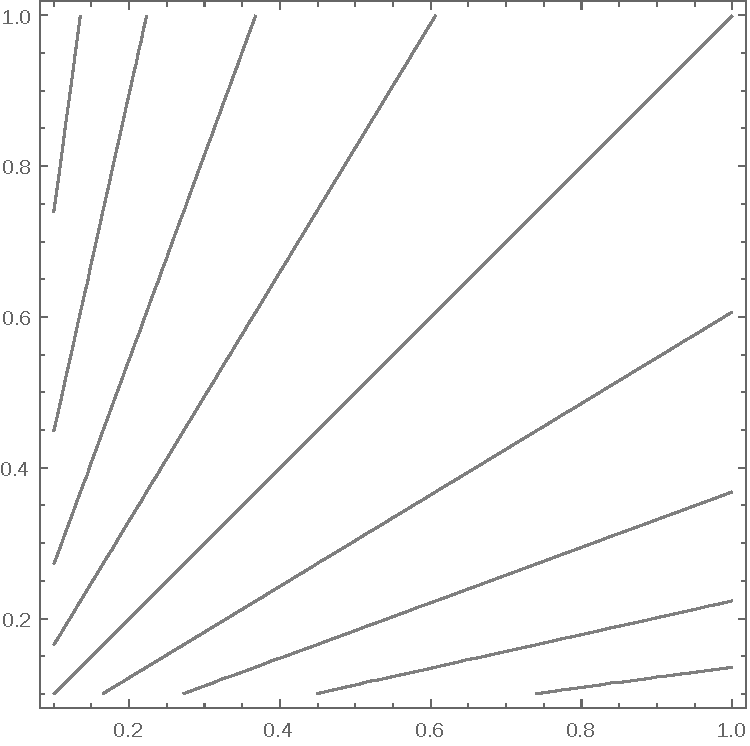
\includegraphics[width=.45\linewidth]{contour_u.pdf}
    \hfill
    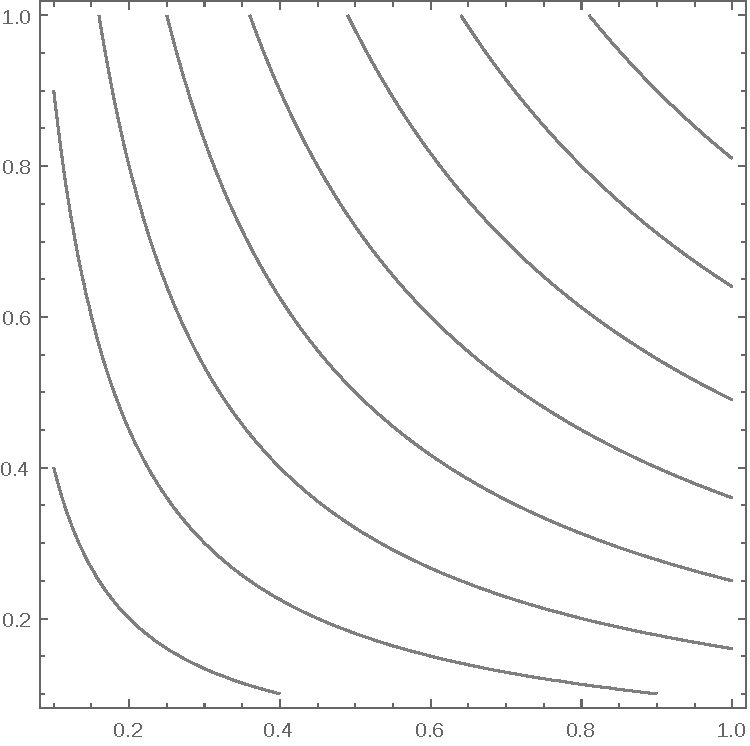
\includegraphics[width=.45\linewidth]{contour_v.pdf}
    \caption{%
        Visualization of $\dif u$ and $\dif v$ as a set of contour lines on
        $\R^2$.
    }
    \label{fig:contour}
\end{figure}

\begin{figure}[htbp]
    \centering
    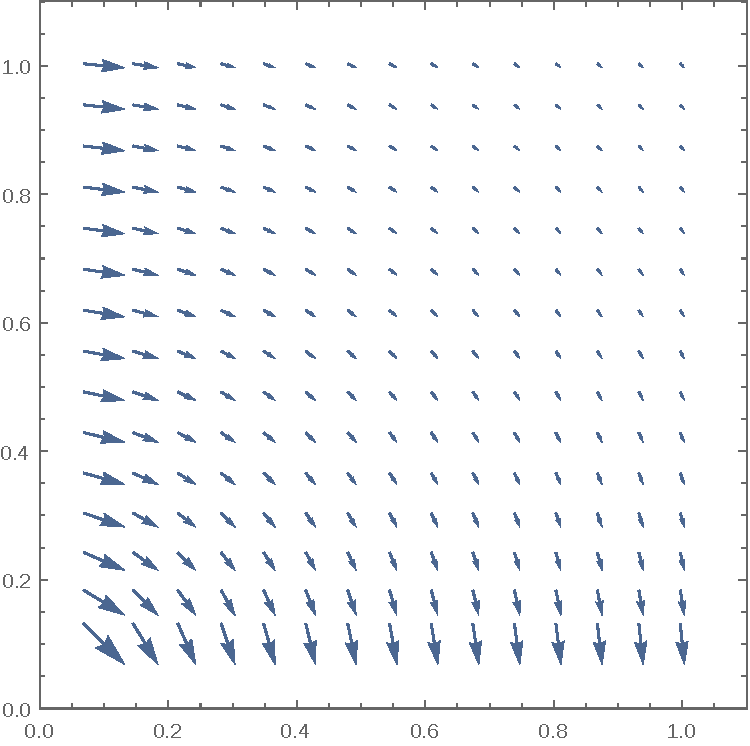
\includegraphics[width=.45\linewidth]{vec_u.pdf}
    \hfill
    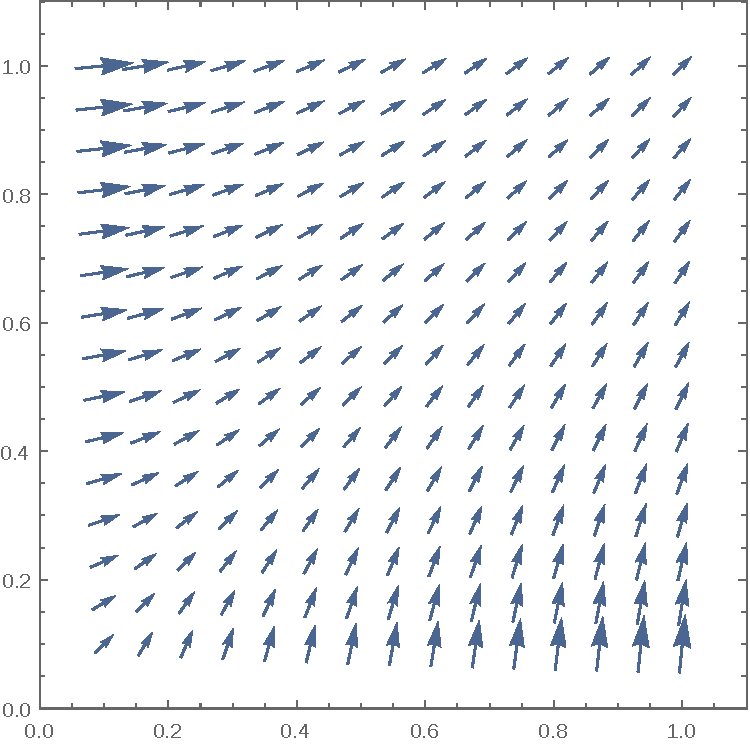
\includegraphics[width=.45\linewidth]{vec_v.pdf}
    \caption{%
        Visualization of $\dif u$ and $\dif v$ as a covector field on
        $[\R^2]^*$.
    }
    \label{fig:covector}
\end{figure}

The 2-form $\dif u \wedge \dif v$ can also be visualized. Since the manifold is
$\R^2$, the space $\Lambda^2 \R^2$ only has one dimension at each point, there
is only one basis vector, $\dif x^1 \wedge \dif x^2$. This means that the
2-form can be visualized as an area density, see Figure~\ref{fig:density}.

\begin{figure}[htbp]
    \centering
    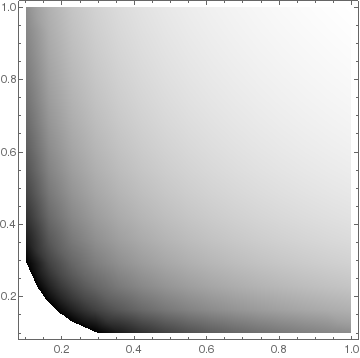
\includegraphics[width=.45\linewidth]{density_uv.png}
    \caption{%
        Visualization of $\dif u \wedge \dif v$ as an area density.
    }
    \label{fig:density}
\end{figure}

\section{Pullback}
\label{homework:4}

\subsection{Linearity}

\begin{align*}
    F^*[\omega + k \theta](\vec v_1, \ldots, \vec v_p)
    &= [\omega + k \theta] \del{F(\vec v_1), \ldots, F(\vec v_p)}
    \intertext{%
        Now we use the linearity in the addition of forms.
    }
    &= \omega\del{F(\vec v_1), \ldots, F(\vec v_p)}
    + k \theta \del{F(\vec v_1), \ldots, F(\vec v_p)}
\end{align*}
And that shows the linearity of the pullback.

\subsection{Product rule}

The pullback is defined by
\begin{align*}
    \sbr{F^*(\omega \wedge \theta)}_{\alpha\ldots\beta\ldots}
    &= [\omega \wedge \theta]_{\gamma\ldots\delta\ldots}
    \pd{F^\gamma}{x^\alpha} \ldots
    \pd{F^\delta}{x^\beta} \ldots.
    \intertext{%
        Using the definition of the wedge product together with the idempotent
        antisymmetrization notation, this can be written explicitly as
    }
    &= \frac{[p+q]!}{p!q!} \omega_{[\gamma\ldots} \theta_{\delta\ldots]}
    \pd{F^\gamma}{x^\alpha} \ldots
    \pd{F^\delta}{x^\beta} \ldots.
    \intertext{%
        The partial derivatives are just plain numbers and commute with
        everything else. It breaks the antisymmetrization notation, but it will
        look like this:
    }
    &= \frac{[p+q]!}{p!q!} \omega_{[\gamma\ldots}
    \pd{F^\gamma}{x^\alpha} \ldots
    \theta_{\delta\ldots]}
    \pd{F^\delta}{x^\beta} \ldots.
    \intertext{%
        Now there are two individual pullbacks. Here the notation works again.
    }
    &= \frac{[p+q]!}{p!q!} [F^*\omega]_{[\gamma\ldots}
    [F^*\theta]_{\delta\ldots]}
    \intertext{%
        This is the definition of the wedge product again. So we can write this
        as the desired form,
    }
    &= \sbr{F^*\omega \wedge F^*\theta}_{\gamma\ldots\delta\ldots}.
\end{align*}
Omitting the indices will give the form given on the problem set.

\subsection{Chain rule}

The definition of the pullback gives
\begin{align*}
    \sbr{[G \circ F]^* \omega}_{\alpha\ldots}
    &= \omega_{\gamma\ldots} \pd{[G \circ F]^\gamma}{x^\alpha} \ldots.
    \intertext{%
        Then we apply the chain rule to the linear maps.
    }
    &= \underbrace{\omega_{\gamma\ldots}
    \pd{G^\gamma}{F^\mu}}_{[G^*\omega]_{\mu\ldots}} \pd{F^\mu}{x^\alpha} \ldots.
    \intertext{%
        We identify the pullback with $G$ there. The whole expression then is
    }
    &= \sbr{F^*[G^*\omega]}_{\alpha\ldots}
    \intertext{%
        or
    }
    &= \sbr{[F^* \circ G^*] \omega}_{\alpha\ldots}.
\end{align*}

\end{document}

% vim: spell spelllang=en tw=79
